
El presente capítulo describe el modelo de estados correspondiente a las entidades de la Escuela Libre de Derecho Posgrado que tiene un comportamiento dinámico en el sistema. Esta conformado por los siguientes elementos:
%Referencias de los modelos en el capitulo
\begin{itemize}
%	\item Modelo del ciclo de vida de un Diplomado, el cual define la evolución de un Diplomado dentro de la ELD.
	\item Modelo del ciclo de vida de un Plan de estudios/Versión, el cual define la evolución de un plan de estudios para especialidad y maestría o una versión para diplomado dentro de la ELD.
%	\item Modelo del ciclo de vida de una Especialidad, el cual define la evolución de una Especialidad dentro de la ELD.
%	\item Modelo del ciclo de vida de una Maestría, el cual define la evolución de una Maestría dentro de la ELD.
\end{itemize}

%========================Modelo de diplomado =============================================

%\hypertarget{cv:Diplomado}{\section{Modelo del ciclo de vida de un Diplomado}}		
%		
%		Un diplomado puede pasar por una serie de etapas o 'estados' en el sistema. Dependiendo del estado en el que se encuentre el diplomado, el actor puede realizar diferentes actividades. Los estados y transiciones se muestran en la figura \ref{fig:MEDiplomado} y se describen a continuación.
%			
%			\begin{figure}[htbp!]
%				\centering
%				\fbox{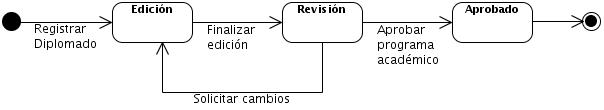
\includegraphics[width=\textwidth]{images/maquinasEstados/MaquinaEstadosPA.jpg}}
%				\caption{Modelo del ciclo de vida de un Diplomado.}
%				\label{fig:MEDiplomado}
%			\end{figure}
%			
%		\noindent \textbf{Edición:} El diplomado toma este estado cuando es registrado o cuando la \cdtRef{Actor:SP}{Secretaría de Posgrado} solicita cambios al mismo. Un diplomado en este estado puede ser editado, se pueden gestionar sus versiones y se puede eliminar, solamente si no tiene versiones registradas. Este estado es el inicio de la transición hacia el estado:	
%		\begin{itemize}
%			\item \textbf{Revisión:} Pasa a este estado cuando la \cdtRef{Actor:CCE}{Coordinación de Control Escolar} o la \cdtRef{Actor:SP}{Secretaría de Posgrado} ha terminado de gestionar la primera versión del diplomado. 
%		\end{itemize}	
%	
%		\noindent \textbf{Revisión:} El diplomado toma este estado cuando la \cdtRef{Actor:CCE}{Coordinación de Control Escolar} o la \cdtRef{Actor:SP}{Secretaría de Posgrado} finaliza la edición del diplomado y de su primera versión. Este estado es el inicio de las transiciones hacia los estados:
%		\begin{itemize}
%			\item \textbf{Edición:} Pasa a este estado cuando la \cdtRef{Actor:SP}{Secretaría de Posgrado} solicita modificaciones en el diplomado o en la primera versión registrada.
%			
%			\item \textbf{Aprobado:} Pasa a este estado cuando la \cdtRef{Actor:SP}{Secretaría de Posgrado} indica que no hay cambios para el diplomado y para su primera versión registrada, validando que la información de ambas es correcta.
%		\end{itemize}
%	
%	\noindent \textbf{Aprobado:}El diplomado toma este estado cuando la \cdtRef{Actor:SP}{Secretaría de Posgrado} aprueba el diplomado y la primera versión del mismo, indicando que la información registrada es correcta. Es un estado terminal, por lo que no genera transiciones a ningún estado.
%	
%\subsection{Comportamiento de Acciones}
%La tabla \ref{tb:habilitarAcciones} \cdtRef{tb:habilitarAcciones}{Acciones para gestionar diplomados}. muestra la forma en que se habilitarán las acciones en la gestión de diplomados. Las acciones se mostrarán dependiendo del estado en el que se encuentre cada diplomado.\\
%
%\begin{table} 
%\begin{center}
%	\begin{tabular}{|l|l|l|l|}
%		\hline
%		Estado/Operación & Editar Diplomado & Gestionar Versiones & Eliminar Diplomado \\
%		\hline \hline
%		Edición & Habilitado & Habilitado & Habilitado\\ \hline
%		Revisión & Inhabilitado & Inhabilitado & Inhabilitado \\ \hline
%		Aprobado & Inhabilitado & Habilitado & Inhabilitado \\ \hline
%	\end{tabular}
%	\caption{Acciones para gestionar diplomados.}
%	\hypertarget{tb:habilitarAcciones}{}
%	\label{tb:habilitarAcciones}
%\end{center}
%\end{table}

%========================Modelo de plan de estudios/versión =============================================

\hypertarget{cv:Version}{\section{Modelo del ciclo de vida de un Plan de estudios/Versión} }

Un plan de estudios o una versión pueden pasar por una serie de etapas o 'estados' en el sistema. Dependiendo del estado en el que se encuentre el plan de estudios para especialidad y maestría o para la versión en caso de ser un diplomado, el actor puede realizar diferentes actividades. Los estados y transiciones se muestran en la figura \ref{fig:MEdeVersion} y se describen a continuación.

\begin{figure}[htbp!]
	\centering
	\fbox{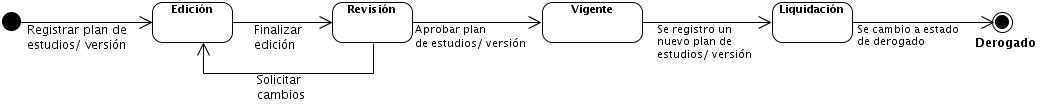
\includegraphics[width=\textwidth]{images/maquinasEstados/MaquinaEstadosV.jpg}}
	\caption{Modelo del ciclo de vida de un Plan de estudios/Versión.}
	\label{fig:MEdeVersion}
\end{figure}

\noindent \textbf{Edición:} Se encuentra en éste estado cuando la \cdtRef{Actor:CCE}{Coordinación de Control Escolar}, la \cdtRef{Actor:DA}{Directora Académica} o la \cdtRef{Actor:SP}{Secretaría de Posgrado} registra un nuevo plan de estudios ya sea para especialidad y maestría o una nueva versión para un diplomado.\\ 

En éste estado, un plan de estudios se puede editar, visualizar, eliminar y finalizar el registro del plan de estudios, así como la gestión de las materias y contenido que contendrá. Una versión se puede editar, visualizar, eliminar y finalizar el registro de una versión, así como la gestión de sus módulos y su contenido.\\

Éste estado es el inicio de la transición hacia el estado:
\begin{itemize}
	\item \textbf{Revisión:} Pasa a este estado una vez que la \cdtRef{Actor:CCE}{Coordinación de Control Escolar}, la \cdtRef{Actor:DA}{Directora Académica} o la \cdtRef{Actor:SP}{Secretaría de Posgrado} ha finalizado el registro del plan de estudios o de una versión, así como sus materias, módulos y contenido de éstos mismos, indicando que la información es correcta y está lista para su revisión.
\end{itemize}

\noindent \textbf{Revisión:} El plan de estudios o la versión pasa a este estado cuando la \cdtRef{Actor:CCE}{Coordinación de Control Escolar}, la \cdtRef{Actor:DA}{Directora Académica} o la \cdtRef{Actor:SP}{Secretaría de Posgrado} manda éste a ser revisado. \\

Éste estado es el inicio de las transiciones hacia los estados:
\begin{itemize}
	\item \textbf{Edición:} Pasa a éste estado cuando la \cdtRef{Actor:SP}{Secretaría de Posgrado} solicita modificaciones en el plan de estudios o la versión.
	
	\item \textbf{Vigente:} Pasa a éste estado cuando la \cdtRef{Actor:SP}{Secretaría de Posgrado} decide aprobar el plan de estudios o la versión, debido a que no requiere cambios, indicando que la información registrada es correcta.
\end{itemize}

\noindent \textbf{Vigente:} El plan de estudios o la versión pasa a éste estado una vez que se aprobó el contenido del plan de estudios o la versión.\\

Éste estado es el inicio de la transición hacia el estado:
\begin{itemize}
	\item \textbf{Liquidación:} El plan de estudios o la versión pasa a éste estado cuando la \cdtRef{Actor:SP}{Secretaría de Posgrado} ha aprobado un nuevo plan de estudios o una nueva versión. 
\end{itemize}

\noindent \textbf{Liquidación:} Se encuentra en éste estado el plan de estudios o la versión que está a punto de ser derogado. Pasan a este estado cuando la  \cdtRef{Actor:SP}{Secretaría de Posgrado} ha aprobado un nuevo plan de estudios o una nueva versión, por lo que el plan de estudios o versión que se encontraba en en estado vigente ha pasado al estado de liquidación.\\

Este estado es el inicio de la transición hacia el estado:
\begin{itemize}
	\item \textbf{Derogado:} El plan de estudios o la versión pasan a éste estado cuando la \cdtRef{Actor:SP}{Secretaría de Posgrado} solicita el cambios de estado de liquidado a derogado. 
\end{itemize} 

\noindent \textbf{Derogado:} El plan de estudios o versión pasa a éste estado cuando la \cdtRef{Actor:SP}{Secretaría de Posgrado} cambia el plan de estudios o la versión al estado derogado, indicando que dicho plan de estudios o dicha versión ya no se impartirá. Este estado no genera transiciones a ningún estado.

\newpage
\subsection{Comportamiento de Acciones}
\href{ComportamientoDeAcciones}{}
\subsubsection{Acciones de la Secretaría de Posgrado para la gestión de planes de estudios/versiones}
La tabla \ref{tb:habilitarAccionesv} \cdtRef{tb:habilitarAccionesv}{Acciones de la secretaría de posgrado para gestionar Planes de estudios/Versiones} muestra la forma en que se habilitarán las acciones para la \cdtRef{Actor:SP}{Secretaría de Posgrado} en la gestión de planes de estudios de maestría y especialidad, de igual manera para las versiones de diplomado. Las acciones se mostrarán dependiendo del estado en el que se encuentre cada plan de estudios y versión.\\
%	\begin{center}
\begin{table}[htpb!] 
\centering
		\begin{tabular}{|c|l|l|l|}
			\hline
			\multicolumn{4}{|c|}{\textbf{Secretaria de Posgrado}} \\
			\hline
			\multicolumn{4}{|c|}{\textbf{Plan de Estudios/Versión}}
			\\ \hline \hline
			\textbf{Estado/Operación} & \textbf{Editar} & \textbf{Visualizar} & \textbf{Gestionar Materias/Módulos} \\ \hline \hline
			Edición & Habilitado & Habilitado & Habilitado \\ \hline
			Revisión & Habilitado & Habilitado & Habilitado \\ \hline
			Vigente & Habilitado & Habilitado & Habilitado \\ \hline
			Liquidación & Habilitado & Habilitado & Habilitado \\ \hline
			Derogado & Inhabilitado & Habilitado & Inhabilitado \\ \hline
		\end{tabular}

\end{table} 
		\begin{table}[htpb!] 

	\centering
	\begin{tabular}{|c|l|l|l|}
		\hline
		\multicolumn{4}{|c|}{\textbf{Secretaria de Posgrado}} \\
		\hline
		\multicolumn{4}{|c|}{\textbf{Plan de Estudios/Versión}}
		\\ \hline \hline
		\textbf{Estado/Operación} & \textbf{Finalizar} & \textbf{Derogar} & \textbf{Eliminar} \\ \hline \hline
		Edición & Habilitado & Inhabilitado & Habilitado \\ \hline
		Revisión & Inhabilitado & Inhabilitado & Habilitado \\ \hline
		Vigente & Inhabilitado & Inhabilitado & Inhabilitado \\ \hline
		Liquidación & Inhabilitado & Habilitado & Inhabilitado \\ \hline
		Derogado & Inhabilitado & Inhabilitado & Inhabilitado \\ \hline
	\end{tabular}
		\caption{Acciones de la secretaría de posgrado para gestionar un plan de Estudios/versión.}
		\hypertarget{tb:habilitarAccionesv}{}
		\label{tb:habilitarAccionesv}
\end{table}
%CCE

\subsubsection{Acciones de la Coordinación de Control Escolar / Directora Académica para la gestión de planes de estudios/versiones}
La tabla \ref{tb:habilitarAccionesvCCE} \cdtRef{tb:habilitarAccionesvCCE}{Acciones de la coordinación de control escolar / Directora Académica para gestionar Planes de estudios/Versiones} muestra la forma en que se habilitarán las acciones para la \cdtRef{Actor:CCE}{Coordinación de Control Escolar} o la \cdtRef{Actor:DA}{Directora Académica} en la gestión de planes de estudios de maestría y especialidad así como versiones de diplomado. Las acciones se mostrarán dependiendo del estado en el que se encuentre cada plan de estudios y versión.\\

\begin{table}[htpb!] 
	\centering
	\begin{tabular}{|c|l|l|l|}
		\hline
		\multicolumn{4}{|c|}{\textbf{Coordinación de Control Escolar / Directora Académica}} \\
		\hline
		\multicolumn{4}{|c|}{\textbf{Plan de Estudios/Versión}}
		\\ \hline \hline
		\textbf{Estado/Operación} & \textbf{Editar} & \textbf{Visualizar} & \textbf{Gestionar Materias/Módulos} \\ \hline \hline
		Edición & Habilitado & Habilitado & Habilitado \\ \hline
		Revisión & Inhabilitado & Habilitado & Inhabilitado \\ \hline
		Vigente & Inhabilitado & Habilitado & Inhabilitado \\ \hline
		Liquidación & Inhabilitado & Habilitado & Inhabilitado \\ \hline
		Derogado & Inhabilitado & Habilitado & Inhabilitado \\ \hline
	\end{tabular}
	
\end{table} 
\begin{table}[htpb!]
	
	\centering
	\begin{tabular}{|c|l|l|l|}
		\hline
		\multicolumn{4}{|c|}{\textbf{Coordinación de Control Escolar / Directora Académica}} \\
		\hline
		\multicolumn{4}{|c|}{\textbf{Plan de Estudios/Versión}}
		\\ \hline \hline
		\textbf{Estado/Operación} & \textbf{Finalizar} & \textbf{Derogar} & \textbf{Eliminar} \\ \hline \hline
		Edición & Habilitado & Inhabilitado & Habilitado \\ \hline
		Revisión & Inhabilitado & Inhabilitado & Inhabilitado \\ \hline
		Vigente & Inhabilitado & Inhabilitado & Inhabilitado \\ \hline
		Liquidación & Inhabilitado & Inhabilitado & Inhabilitado \\ \hline
		Derogado & Inhabilitado & Inhabilitado & Inhabilitado \\ \hline
	\end{tabular}
	\caption{Acciones de la coordinación de control escolar/ directora académica para gestionar plan de estudios/versiones.}
	\hypertarget{tb:habilitarAccionesvCCE}{}
	\label{tb:habilitarAccionesvCCE}
\end{table}


\subsubsection{Acciones de la Secretaría de Posgrado para la gestión del contenido del Plan de estudios/Versión}
La tabla \ref{tb:habilitarAccionesEditar} \cdtRef{tb:habilitarAccionesEditar}{Acciones de la secretaría de posgrado para gestionar el contenido de un plan de estudios/versión} muestra las acciones que podrá realizar la \cdtRef{Actor:SP}{Secretaría de Posgrado} en la gestión de materias, materias derivadas, temas y subtemas de un plan de estudios de especialidad; materias, temas y subtemas de un plan de estudios de maestría y módulos, temas y subtemas de una versión de diplomado dependiendo del estado de dicho plan de estudios o versión.

\begin{table}[htpb!]
	\centering
	\begin{tabular}{|c|l|l|l|}
		\hline
		\multicolumn{4}{|c|}{\textbf{Secretaria de Posgrado}}\\
		\hline
		\multicolumn{4}{|c|}{\textbf{Contenido}}
		\\ \hline \hline
		\textbf{Estado/Operación} & \textbf{Registrar} & \textbf{Editar} & \textbf{Eliminar} \\ \hline \hline
		Edición & Habilitado & Habilitado & Habilitado \\ \hline
		Revisión & Habilitado & Habilitado & Habilitado \\ \hline
		Vigente & Inhabilitado & Habilitado & Inhabilitado \\ \hline
		Liquidación & Inhabilitado & Habilitado & Inhabilitado \\ \hline
		Derogado & Inhabilitado & Inhabilitado & Inhabilitado \\ \hline
	\end{tabular}
	\caption{Acciones de la secretaría de posgrado para gestionar el contenido del plan de estudios/versión.}
	\hypertarget{tb:habilitarAccionesEditar}{}
	\label{tb:habilitarAccionesEditar}
\end{table}
%CCE
\subsubsection{Acciones de la Coordinación de Control Escolar / Directora Académica para la gestión del contenido del Plan de estudios/Versión}
La tabla \ref{tb:habilitarAccionesEditarCCE} \cdtRef{tb:habilitarAccionesEditarCCE}{Acciones de la coordinación de control escolar/ directora académica para gestionar el contenido plan de estudios/versión} muestra las acciones que podrá realizar la \cdtRef{Actor:CCE}{Coordinación de Control Escolar} o la \cdtRef{Actor:DA}{Directora Académica} en la gestión de materias, materias derivadas, temas y subtemas de un plan de estudios de especialidad; materias, temas y subtemas de un plan de estudios de maestría y módulos, temas y subtemas de una versión de diplomado dependiendo del estado de dicho plan de estudios o versión.
\begin{table}[htpb!]
	\centering
	\begin{tabular}{|c|l|l|l|}
		\hline
		\multicolumn{4}{|c|}{\textbf{Coordinación de Control Escolar / Directora Académica}}\\
		\hline
		\multicolumn{4}{|c|}{\textbf{Contenido}}
		\\ \hline \hline
		\textbf{Estado/Operación} & \textbf{Registrar} & \textbf{Editar} & \textbf{Eliminar} \\ \hline \hline
		Edición & Habilitado & Habilitado & Habilitado \\ \hline
		Revisión & Inhabilitado & Inhabilitado & Inhabilitado \\ \hline
		Vigente & Inhabilitado & Inhabilitado & Inhabilitado \\ \hline
		Liquidación & Inhabilitado & Inhabilitado & Inhabilitado \\ \hline
		Derogado & Inhabilitado & Inhabilitado & Inhabilitado \\ \hline
	\end{tabular}
	\caption{Acciones de la coordinación de control escolar/directora académica para gestionar el contenido del Plan de estudios/Versión.}
	\hypertarget{tb:habilitarAccionesEditarCCE}{}
	\label{tb:habilitarAccionesEditarCCE}
\end{table}



%========================Modelo grupo =============================================

\hypertarget{cv:Grupo}{\section{Modelo del ciclo de vida de un Grupo} }

Un grupo puede pasar por una serie de etapas o 'estados' en el sistema. Dependiendo del estado en el que se encuentre el grupo, el actor puede realizar diferentes actividades. Los estados y transiciones se muestran en la figura \ref{fig:MEgrupo} y se describen a continuación.\\


\begin{figure}[htbp!]
	\centering
	\fbox{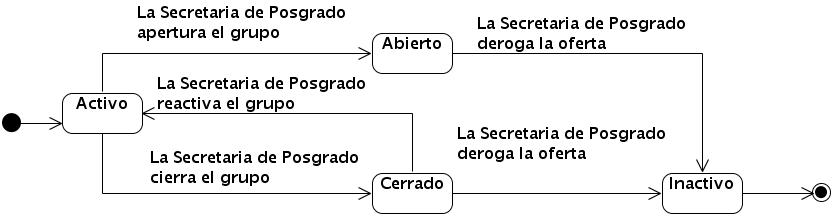
\includegraphics[width=\textwidth]{images/maquinasEstados/MaquinaEstadosGrupo.jpg}}
	\caption{Modelo del ciclo de vida de un Grupo.}
	\label{fig:MEgrupo}
\end{figure}

\noindent \textbf{Activo:} Se encuentra en éste estado cuando la \cdtRef{Actor:SP}{Secretaria de Posgrado} pone en vigente la oferta del programa académico de  Especialidad, Maestría o Diplomado que está asociado al grupo. En éste estado, un grupo se puede abrir o cerrar, así como inscribir aspirantes al grupo o anular dicha inscripción.\\

Éste estado es el inicio de las transiciones hacia los estados:
\begin{itemize}
	\item \textbf{Abierto:} Pasa a éste estado cuando la \cdtRef{Actor:SP}{Secretaria de Posgrado} decide abrir un grupo asociado al programa académico.	
	\item \textbf{Cerrado:} Pasa a éste estado cuando la \cdtRef{Actor:SP}{Secretaria de Posgrado} decide cerrar un grupo asociado al programa académico.
\end{itemize}

\noindent \textbf{Abierto:} El grupo pasa a este estado cuando la \cdtRef{Actor:SP}{Secretaria de Posgrado} lo apertura con la finalidad de que el programa académico asociado sea impartido. En éste estado, a un grupo se le puede finalizar la inscripción de aspirantes o anular la inscripción de alguno.\\

Éste estado es el inicio de la transición hacia el estado:
\begin{itemize}
	\item \textbf{Inactivo:} Pasa a éste estado cuando la \cdtRef{Actor:SP}{Secretaria de Posgrado} deroga la oferta del programa académico.	
\end{itemize}

\noindent \textbf{Cerrado:} El grupo pasa a este estado cuando la \cdtRef{Actor:SP}{Secretaria de Posgrado} lo cierra, esto quiere decir que no se podrá impartir el programa académico en los grupos que se encuentren en éste estado.\\

%Los programas académicos que se encuentren asociados a los grupos en este estado cerrado, no podrán impartirse en estos grupos.
%En los grupos que se encuentren en éste estado no se impartirá el programa académico asociado.
%, indicando que el grupo cerrado no se impartirá el programa académico asociado. En éste estado, un grupo solo se puede reactivar.\\

Éste estado es el inicio de las transiciones hacia los estados:
\begin{itemize}
	\item \textbf{Activo:} Pasa a éste estado cuando la \cdtRef{Actor:SP}{Secretaria de Posgrado} decide reactivar un grupo.	
	\item \textbf{Inactivo:} Pasa a éste estado cuando la \cdtRef{Actor:SP}{Secretaria de Posgrado} deroga la oferta del programa académico.	
\end{itemize}

\noindent \textbf{Inactivo:} El grupo pasa a este estado cuando la \cdtRef{Actor:SP}{Secretaria de Posgrado} deroga la oferta del programa académico. Éste estado no genera transiciones a ningún estado.


%========================Modelo aspirante =============================================

\hypertarget{cv:Aspirante}{\section{Modelo del ciclo de vida de un Aspirante} }

Un aspirante puede pasar por una serie de etapas o 'estados' en el sistema. Dependiendo del estado en el que se encuentre el aspirante, puede realizar diferentes actividades. Los estados y transiciones se muestran en la figura \ref{fig:MEaspirante} y se describen a continuación.\\

\begin{figure}[htbp!]
	\centering
	\fbox{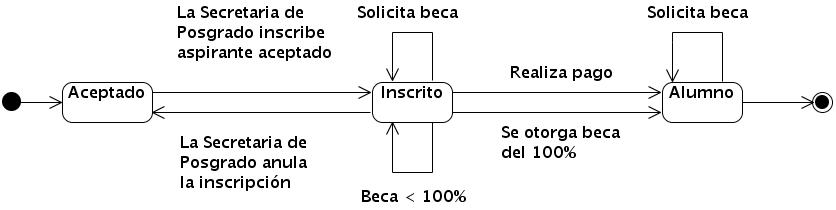
\includegraphics[width=\textwidth]{images/maquinasEstados/MaquinaEstadosAspirante.jpg}}
	\caption{Modelo del ciclo de vida de un Aspirante.}
	\label{fig:MEaspirante}
\end{figure}

\noindent \textbf{Aceptado:} Se encuentra en éste estado cuando un \cdtRef{Actor:AspiranteAceptado}{aspirante} aprueba todas y cada una de las etapas de admisión. En éste estado puede ser inscrito en un grupo del programa académico al que fue candidato.\\

Éste estado es el inicio de la transición hacia el estado:
\begin{itemize}
	\item \textbf{Inscrito:} Pasa a éste estado cuando la \cdtRef{Actor:SP}{Secretaria de Posgrado} inscribe al \cdtRef{Actor:AspiranteAceptado}{aspirante} en un grupo del programa académico al que participó.	
\end{itemize}

\noindent \textbf{Inscrito:} El aspirante pasa a este estado cuando la \cdtRef{Actor:SP}{Secretaria de Posgrado} lo inscribe en un grupo del programa académico al que se registró. En éste estado un aspirante puede realizar el pago de su inscripción o en su defecto solicitar una beca. \\

Éste estado es el inicio de las transiciones hacia los estados:
\begin{itemize}
	\item \textbf{Inscrito:} Pasa a éste estado cuando realiza la solicitud de beca, cuando ésta es rechazada o cuando el porcentaje de la beca otorgada es menor al 100\%.
	\item \textbf{Aceptado:} Pasa a éste estado cuando la \cdtRef{Actor:SP}{Secretaria de Posgrado} anula la inscripción del \cdtRef{Actor:AspiranteAceptado}{aspirante}.
	\item \textbf{Alumno:} Pasa a éste estado cuando realiza el pago de su inscripción o en su defecto le es otorgada una beca del 100\%.	
\end{itemize}

\noindent \textbf{Alumno:} El aspirante pasa a este estado cuando realiza el pago de su inscripción o en su defecto le es otorgada una beca del 100\%. En éste estado, un alumno puede solicitar beca, en el caso de que no haya solicitado beca o que su solicitud haya sido rechazada anteriormente.\\

Éste estado es el inicio de la transición hacia el estado:
\begin{itemize}
	\item \textbf{Alumno:} Pasa a éste estado cuando realiza la solicitud de beca.	
\end{itemize}

Este es es el estado final de un aspirante.
